\subsubsection{TCM\cite{tang_graph_2016}}

\paragraph{}
Approximate Frequency Count sketches store aggregated frequencies of edges in summarized form. When there is a graph stream as indicated in \autoref{fig:afc_sample_stream}, its summarized node sketch and edge sketch would be the mappings described by \autoref{fig:afc_node_sketch} and \autoref{fig:afc_edge_sketch} respectively.

\begin{figure}[H]
    \centering 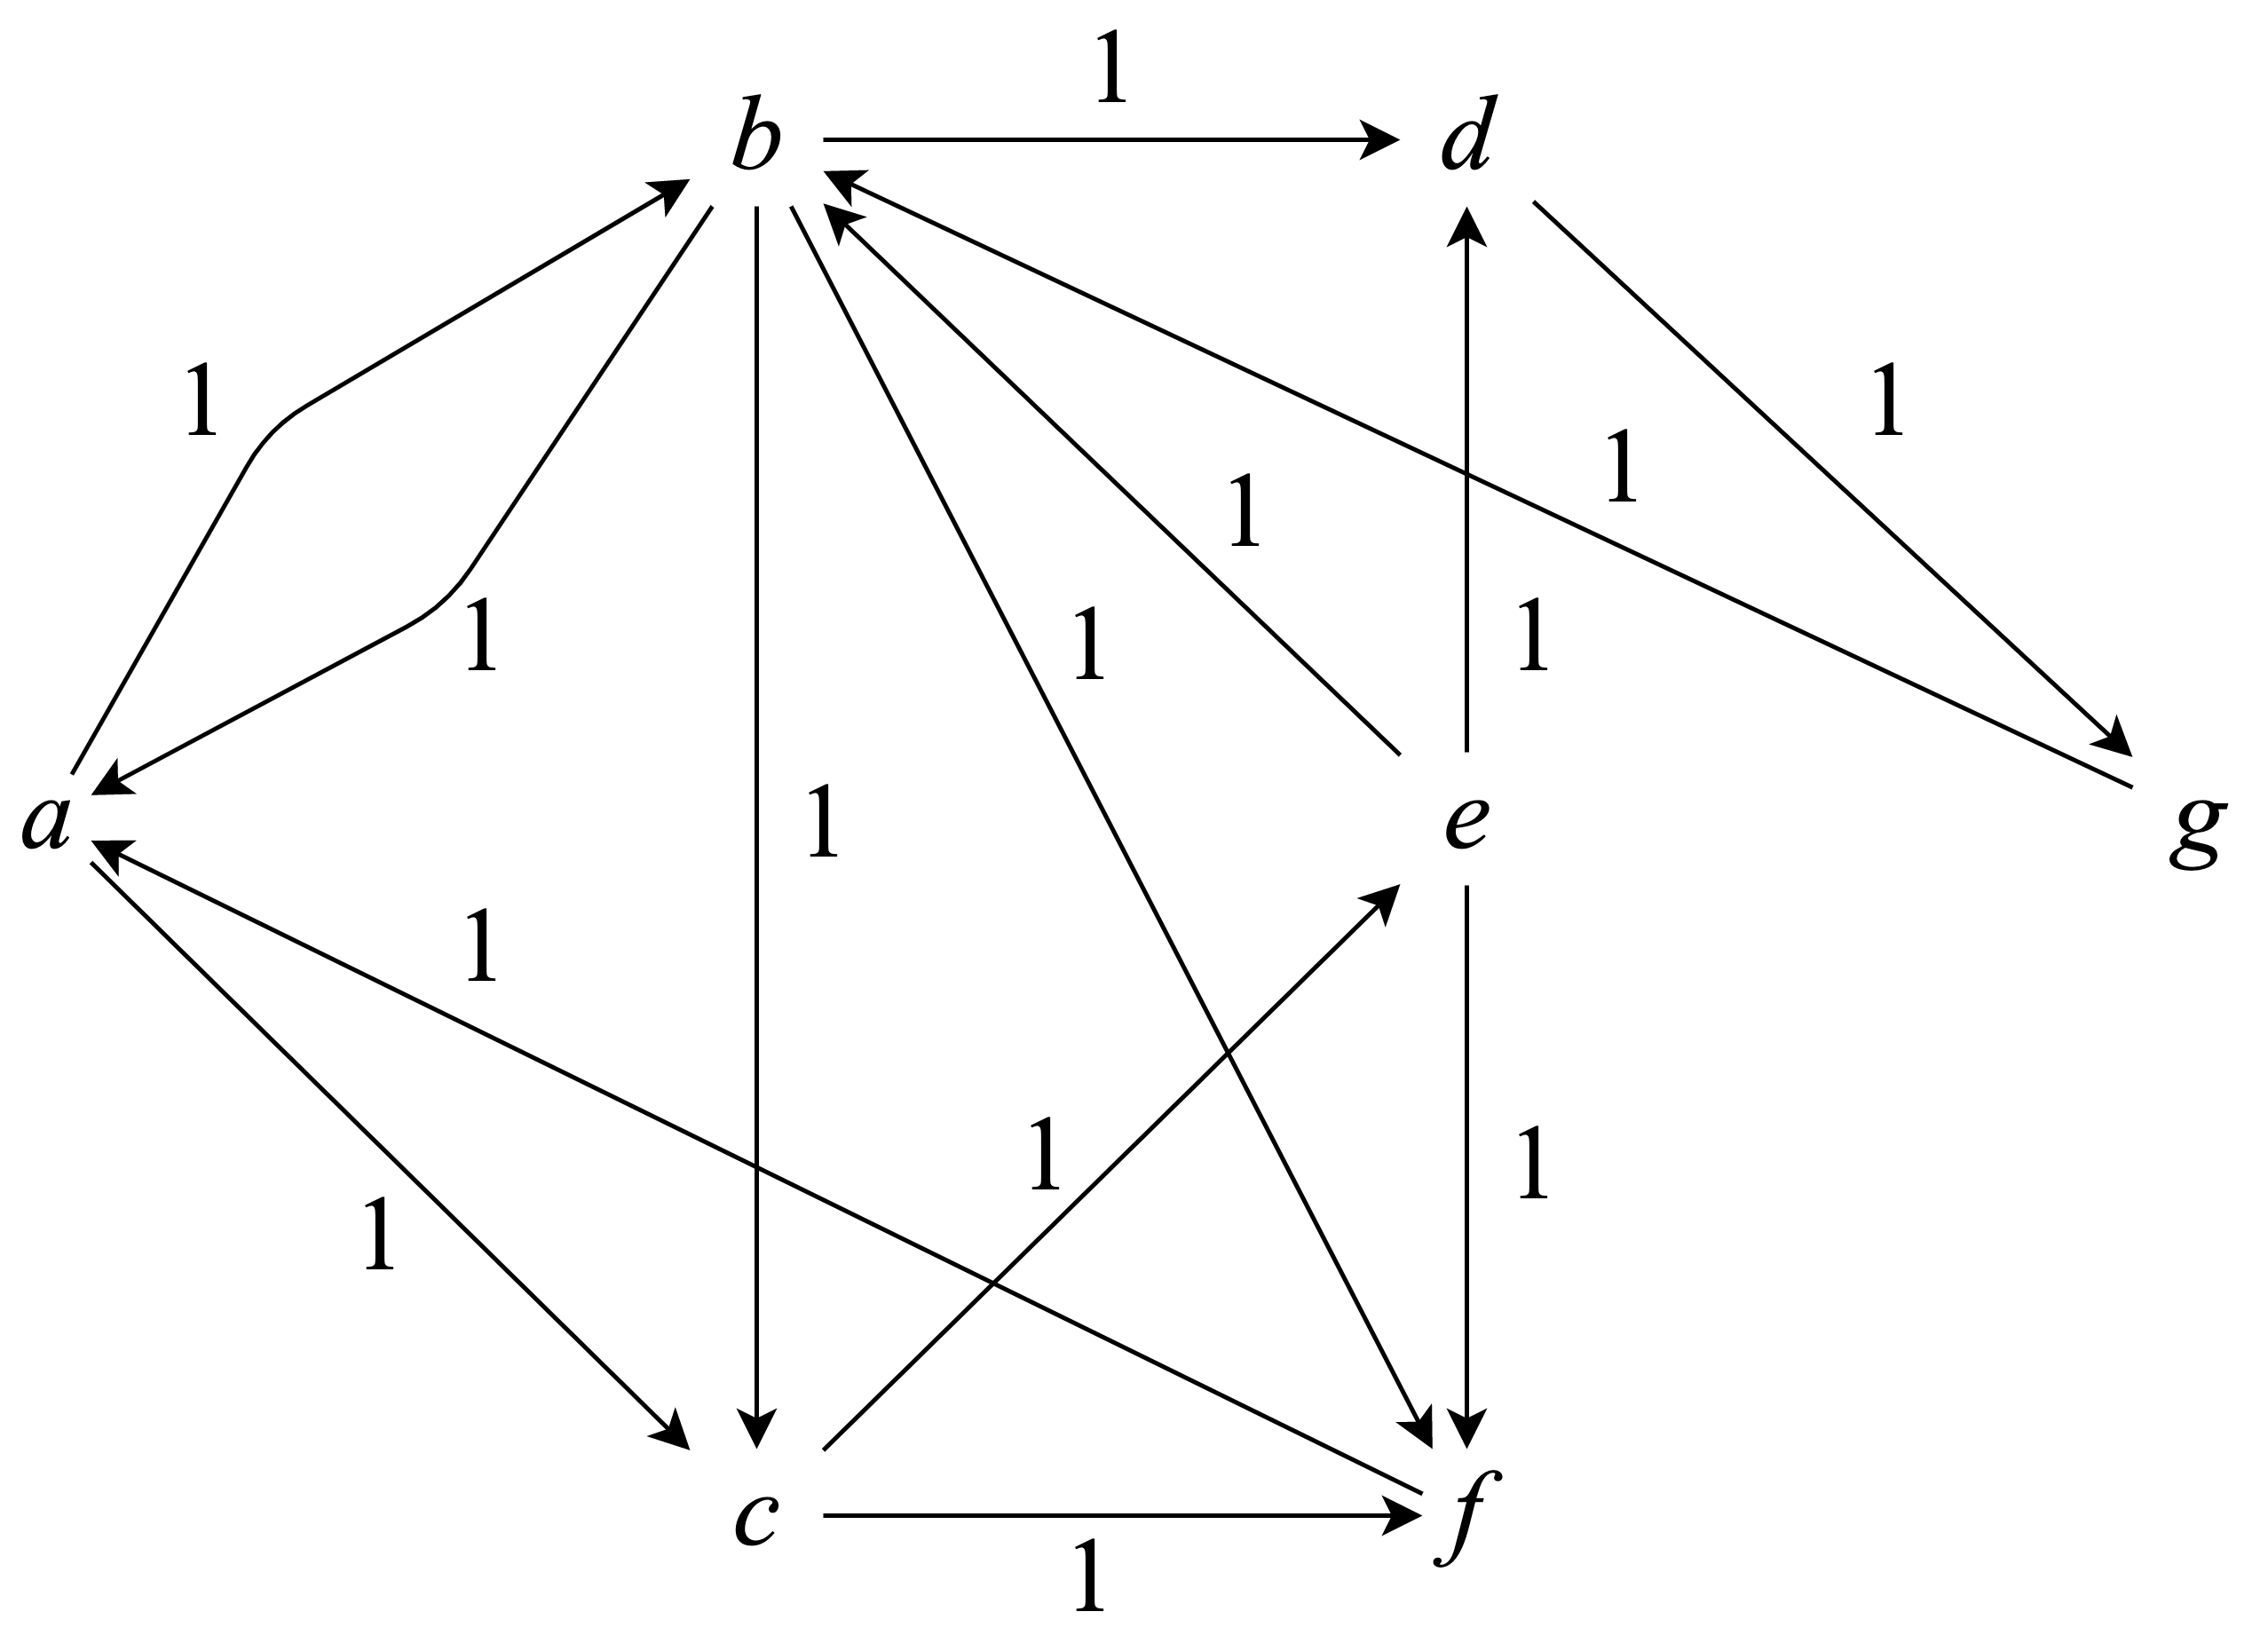
\includegraphics[width=0.5\textwidth]{afc_sample_stream}
    \caption{A sample graph stream}
    \label{fig:afc_sample_stream}
\end{figure}

\begin{figure}[H]
    \centering 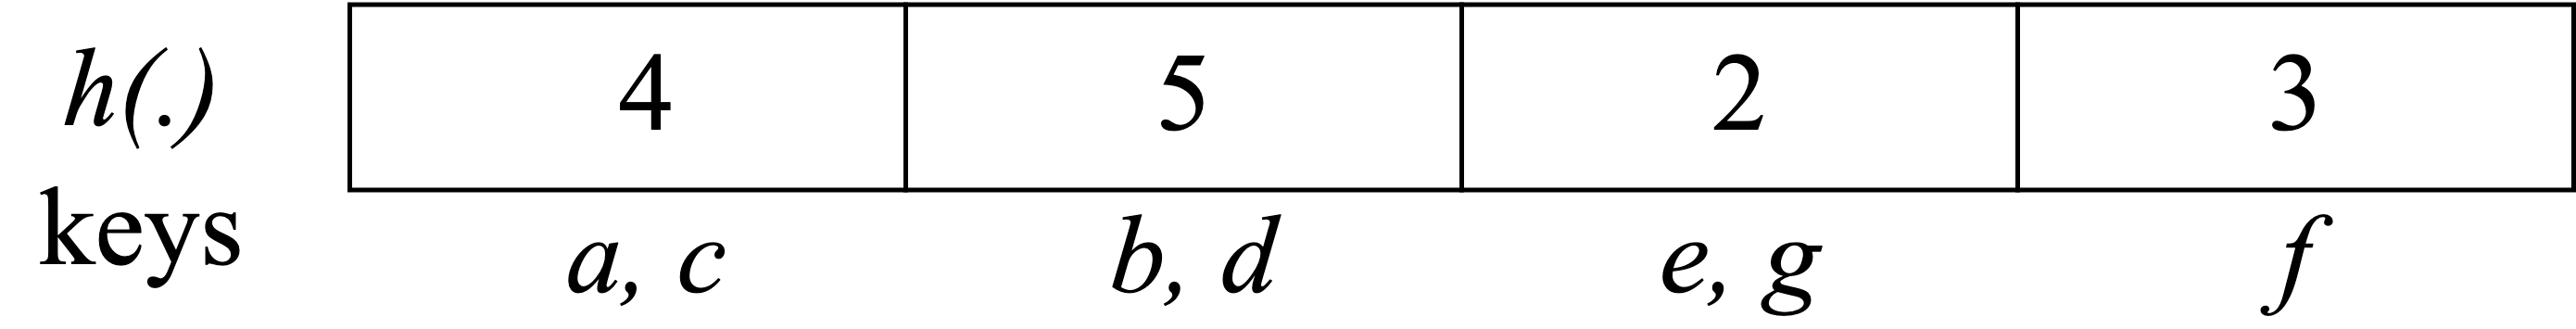
\includegraphics[width=0.5\textwidth]{afc_node_sketch}
    \caption{Node sketch}
    \label{fig:afc_node_sketch}
\end{figure}

\begin{figure}[H]
    \centering 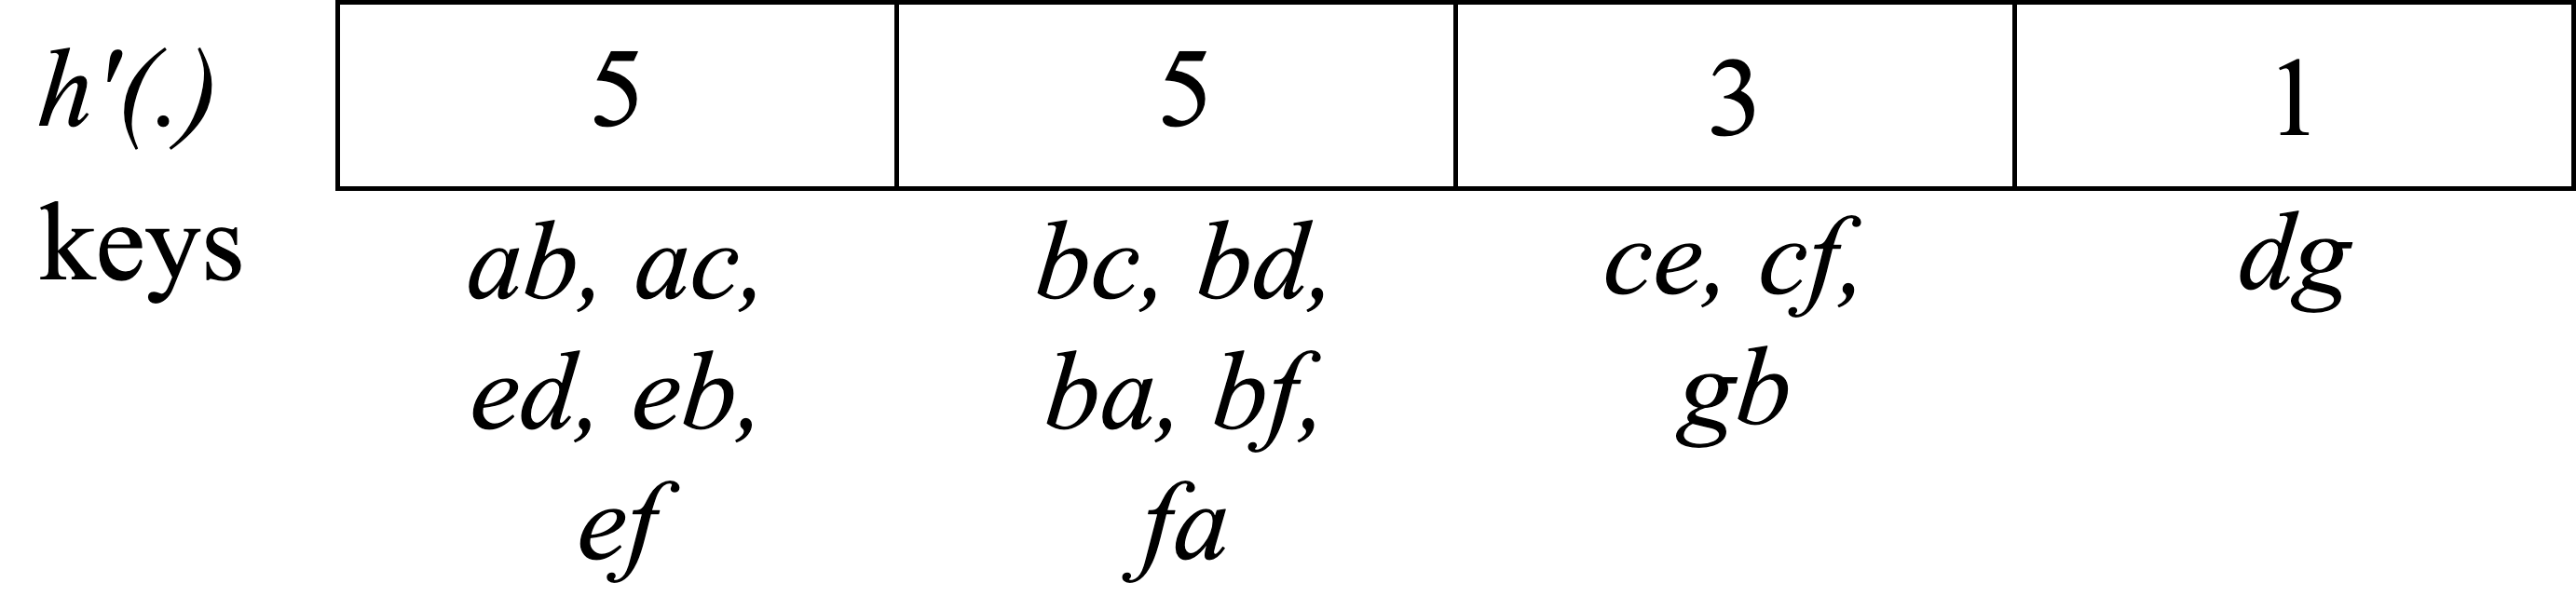
\includegraphics[width=0.5\textwidth]{afc_edge_sketch}
    \caption{Edge sketch}
    \label{fig:afc_edge_sketch}
\end{figure}

\paragraph{}
A disadvantage posed by all the approximate frequency count sketches like CountMin or gSketch is that they do not store the locality of the nodes. Therefore they cannot be used for conditional node queries or queries involving node connectivity. If these queries were to be run, at least some of the information about the locality of nodes has to be retained in the graph synopses. TCM can summarize both node and edge information in constant time. Because of that, it can answer a wide range of queries, unlike its predecessors. The structure of a TCM sketch is depicted in \autoref{fig:tcm}.

\begin{figure}[H]
    \centering 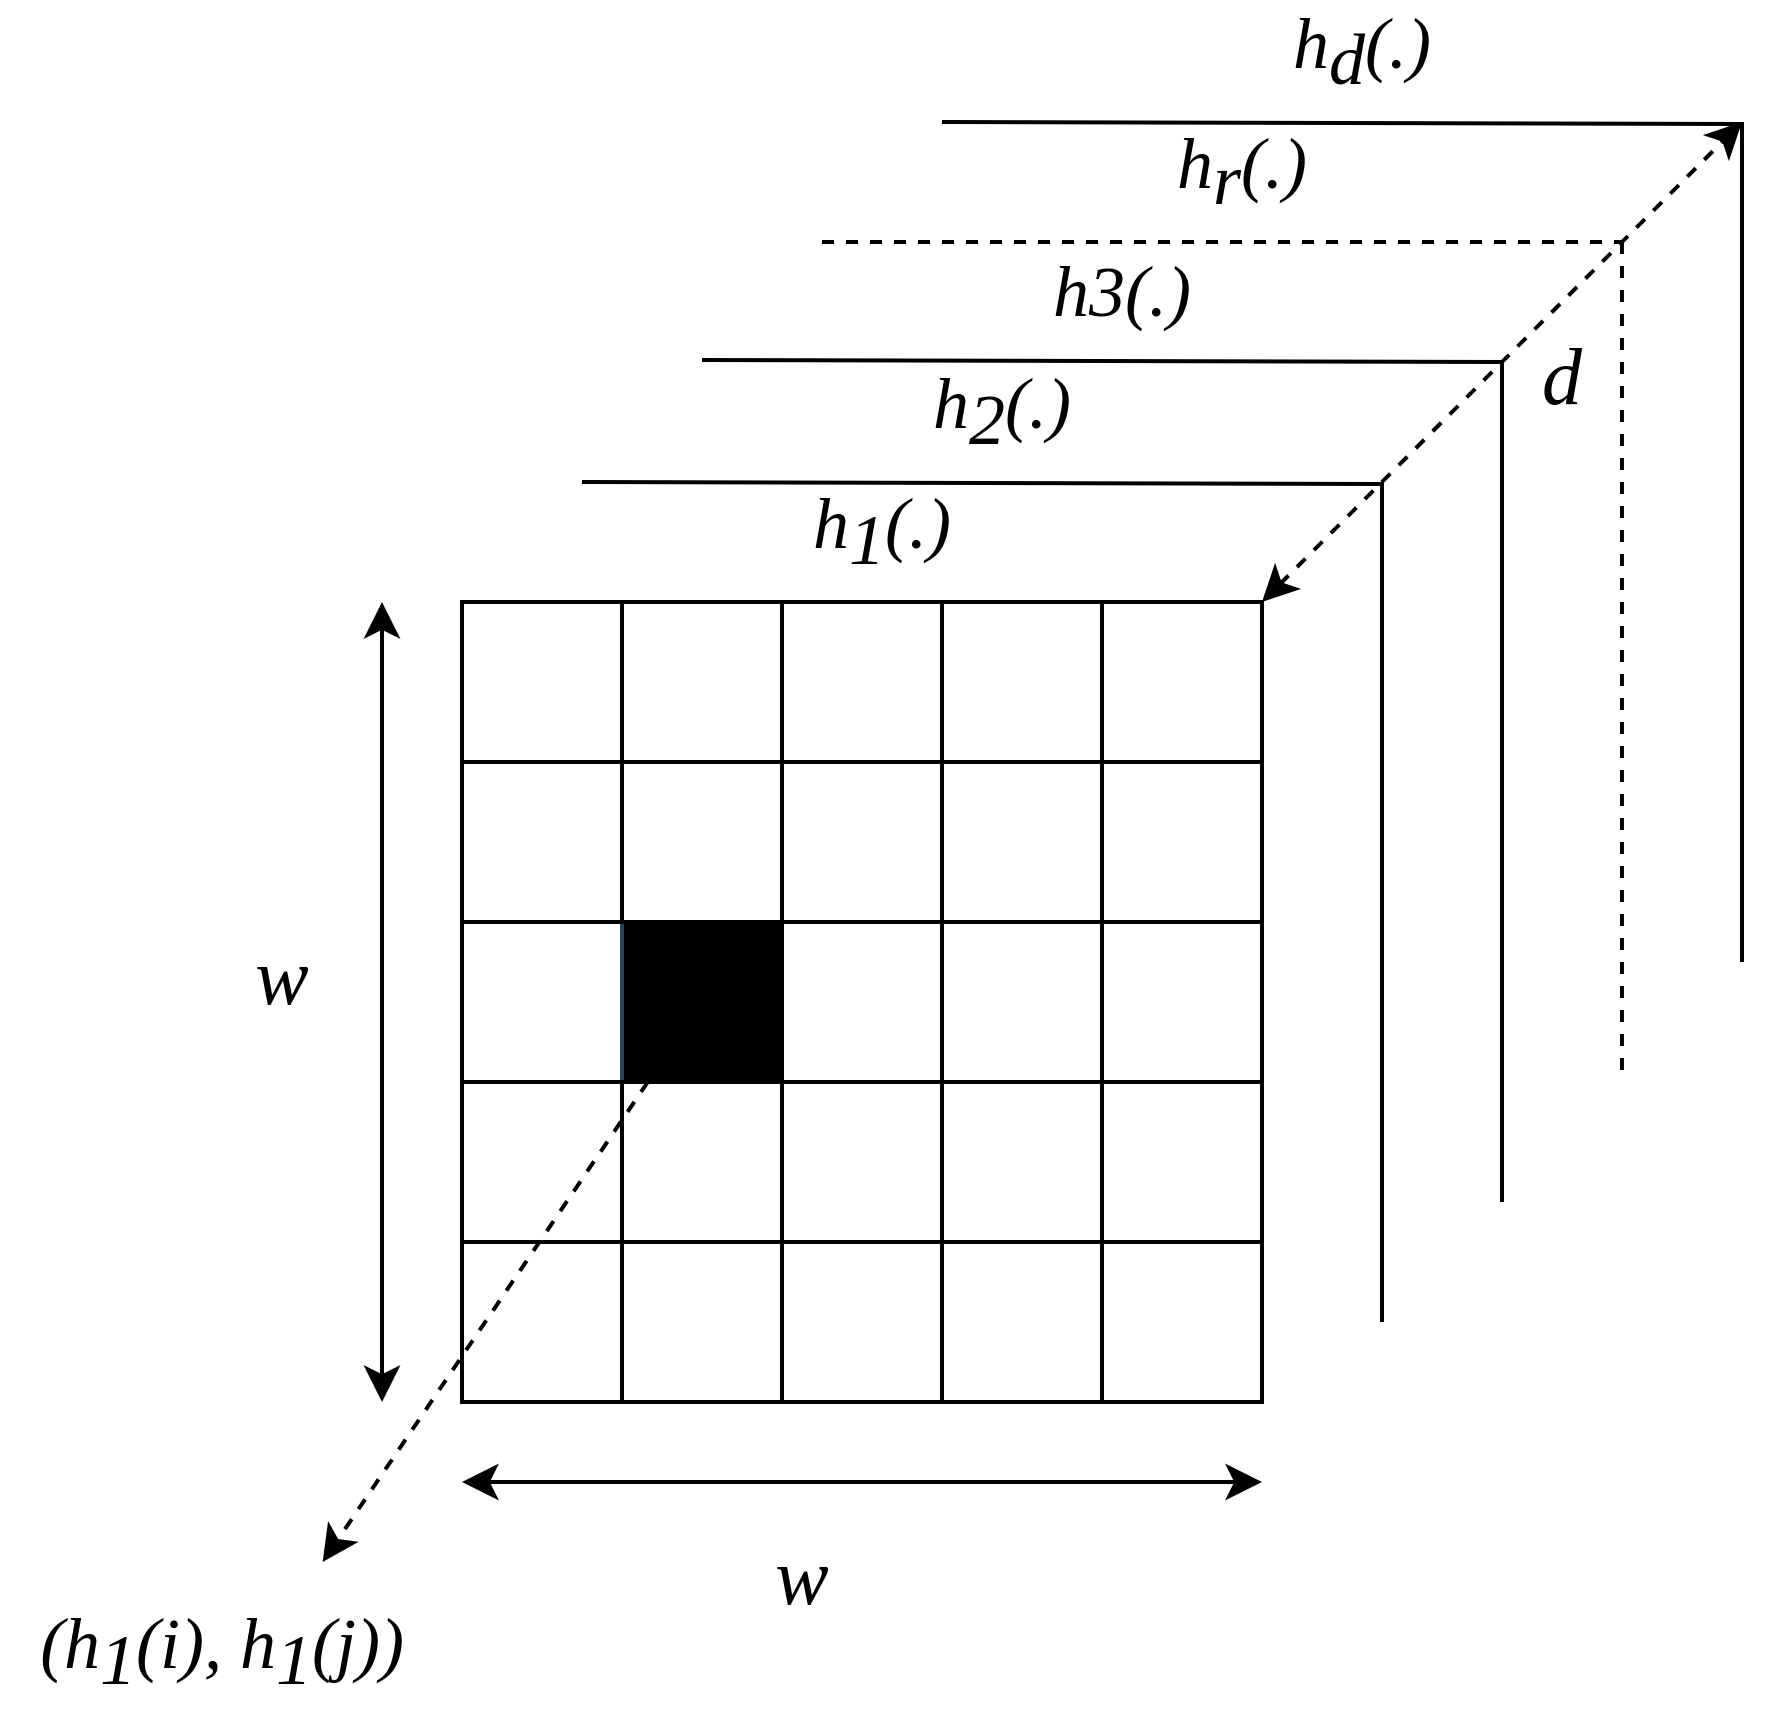
\includegraphics[width=0.7\textwidth]{tcm}
    \caption{TCM sketch}
    \label{fig:tcm}
\end{figure}